\documentclass[a4paper,twoside]{article}

\usepackage{epsfig}
\usepackage{subfigure}
\usepackage{calc}
\usepackage{amssymb}
\usepackage{amstext}
\usepackage{amsmath}
\usepackage{amsthm}
\usepackage{multicol}
\usepackage{url}
\usepackage{booktabs}
\usepackage{tabularx}
\usepackage{cleveref}
\usepackage{pslatex}
\usepackage{apalike}
\usepackage{lipsum}
\usepackage{SCITEPRESS}     % Please add other packages that you may need BEFORE the SCITEPRESS.sty package.

\subfigtopskip=0pt
\subfigcapskip=0pt
\subfigbottomskip=0pt

\begin{document}
	
\title{Title of your Team Project  \subtitle{CIS4010 Cloud Computing Team Project Report} }
	
\author{\authorname{Tyler Green, and Team Member 2}
	\affiliation{School of Computer Science, University of Guelph, Guelph, Ontario, Canada}
	\email{\{tgreen10, email2\}@uoguelph.ca}
}
	
\keywords{Azure, Speech Recognition, keyword3, keyword4}
	
\abstract{This is a short description of the contents of this report. Briefly describe the project goals and results.  In this template you will find all the sections and subsections that definitely must appear in your report.  You will also find all of the information that you need to create a LaTeX document that corresponds to the required project report format.  There are many sites on the Internet that can help you with LaTeX and BibTex (the citation/referencing part of the document) so Google away to find out anything that I have not included in this template.  This template does show examples of image insertion and citation of references and parts of the document itself (such as figures and sections).}

\onecolumn \maketitle \normalsize \vfill

\section{\uppercase{Introduction}}
\label{sec:introduction}

\noindent In this section you describe the project motivations, goals, and any other information that the reader will need to understand the rest of the report. Be sure to include a brief discussion about why you selected both this project and the approach you used in the project.  At the end of this section you will have a subsection that contains a concise statement of your project's purpose.

\subsection{Project Statement}
\label{sec:statement}

\noindent We aim to help identify the best Speech To Text cloud service out of the services
provided by Azure, AWS. This can be used to help determine what speech
recognition service has the best recognition algorithm for different accents as well as speech
impediments. The best provider will be determined by accuracy, cost, implementation,
performance.

\section{\uppercase{Objectives}}
\label{sec:objectives}

\noindent This is an expansion of the project statement where you explain the goals/objectives of your project. This could include such topics as:
\begin{itemize}
	\item What did you hope to achieve in this project?
	\item What were your educational goals ({\it i.e.} did you use a cloud service that you did not know much about so that you could become more informed about it?)?
	\item Did you want to compare similar services on different platforms?
	\item Did you want to compare using cloud services to non-cloud approaches?
	\item Did you have specific metrics or performance goals?
\end{itemize}

\section{\uppercase{Cloud Aspects}
\label{sec:cloudaspects}}

\noindent This section has an educational focus.  You need to explain the cloud services, tools, platforms, etc. that you used in the project.  Develop a series of brief tutorials (with references) about each cloud service, tool, etc. that you used in this project.  

\subsection{Tutorial Azure Cognitive Services: Speech}
\label{sec:azure}

\noindent Each tutorial topic should be in its own subsection.  This will help the reader appreciate each of the cloud services that you had to handle.

Please include any figures that help with your explanations.  If you do include diagrams, images, or figures from other materials please reference them correctly in the caption of the figure.  Figure \ref{fig:class} shows how this is done.

\begin{figure}
	\caption{Process Types.  Taken from the paper \cite{Cummings2017} }\label{fig:class}
	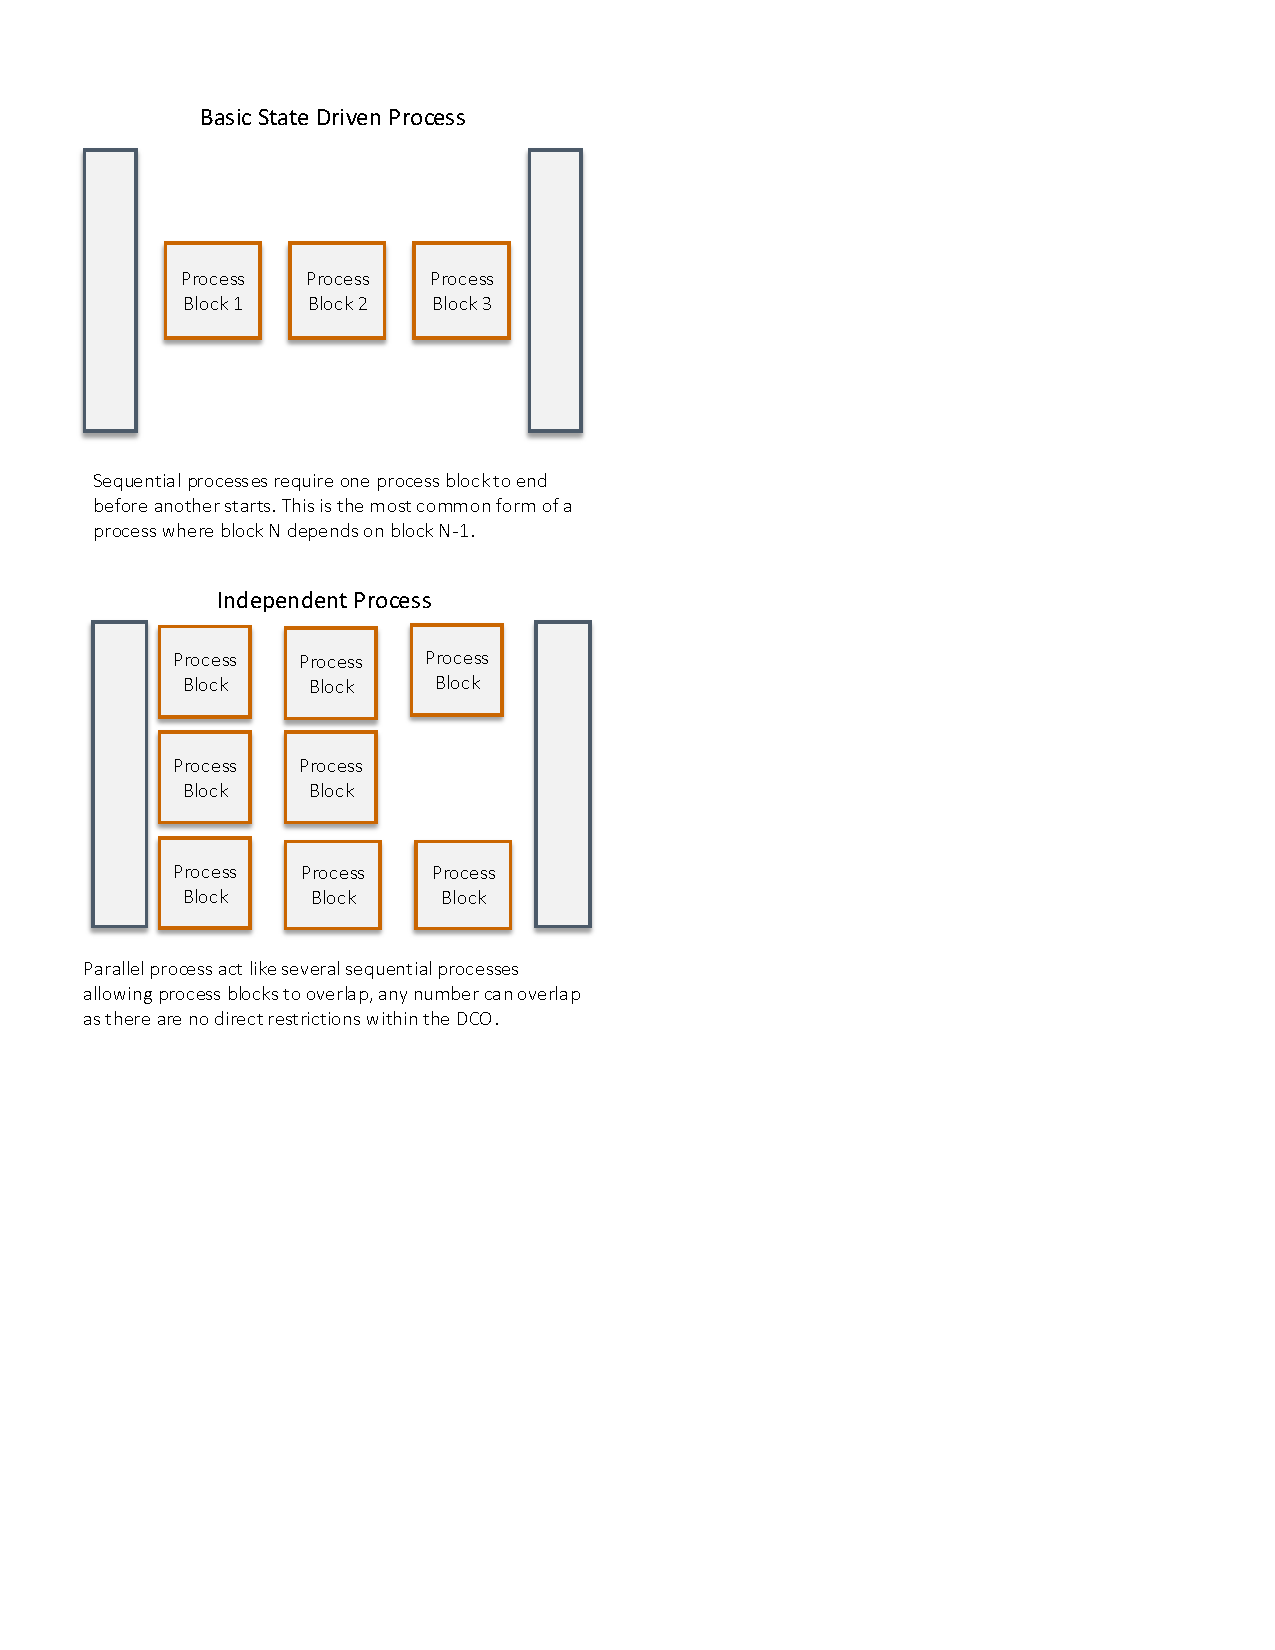
\includegraphics[width=\linewidth]{Images/ProcessTypes}
\end{figure}

If your figure is too wide to fit into the 2 column format of this report, it can still be inserted.  The LaTeX instructions to do so are demonstrated in Figure \ref{fig:vehicles}.  LaTeX decides where it will place your figures.  You can adjust this but sometimes it is very difficult to do, so do not waste your time trying to battle LaTeX; just accept its decisions.

\begin{figure*}[ht]
        \centering
        \caption{The Vehicle Ontology is an example of a wide figure. Taken from \cite{Cummings2017}}
        \label{fig:vehicles}
        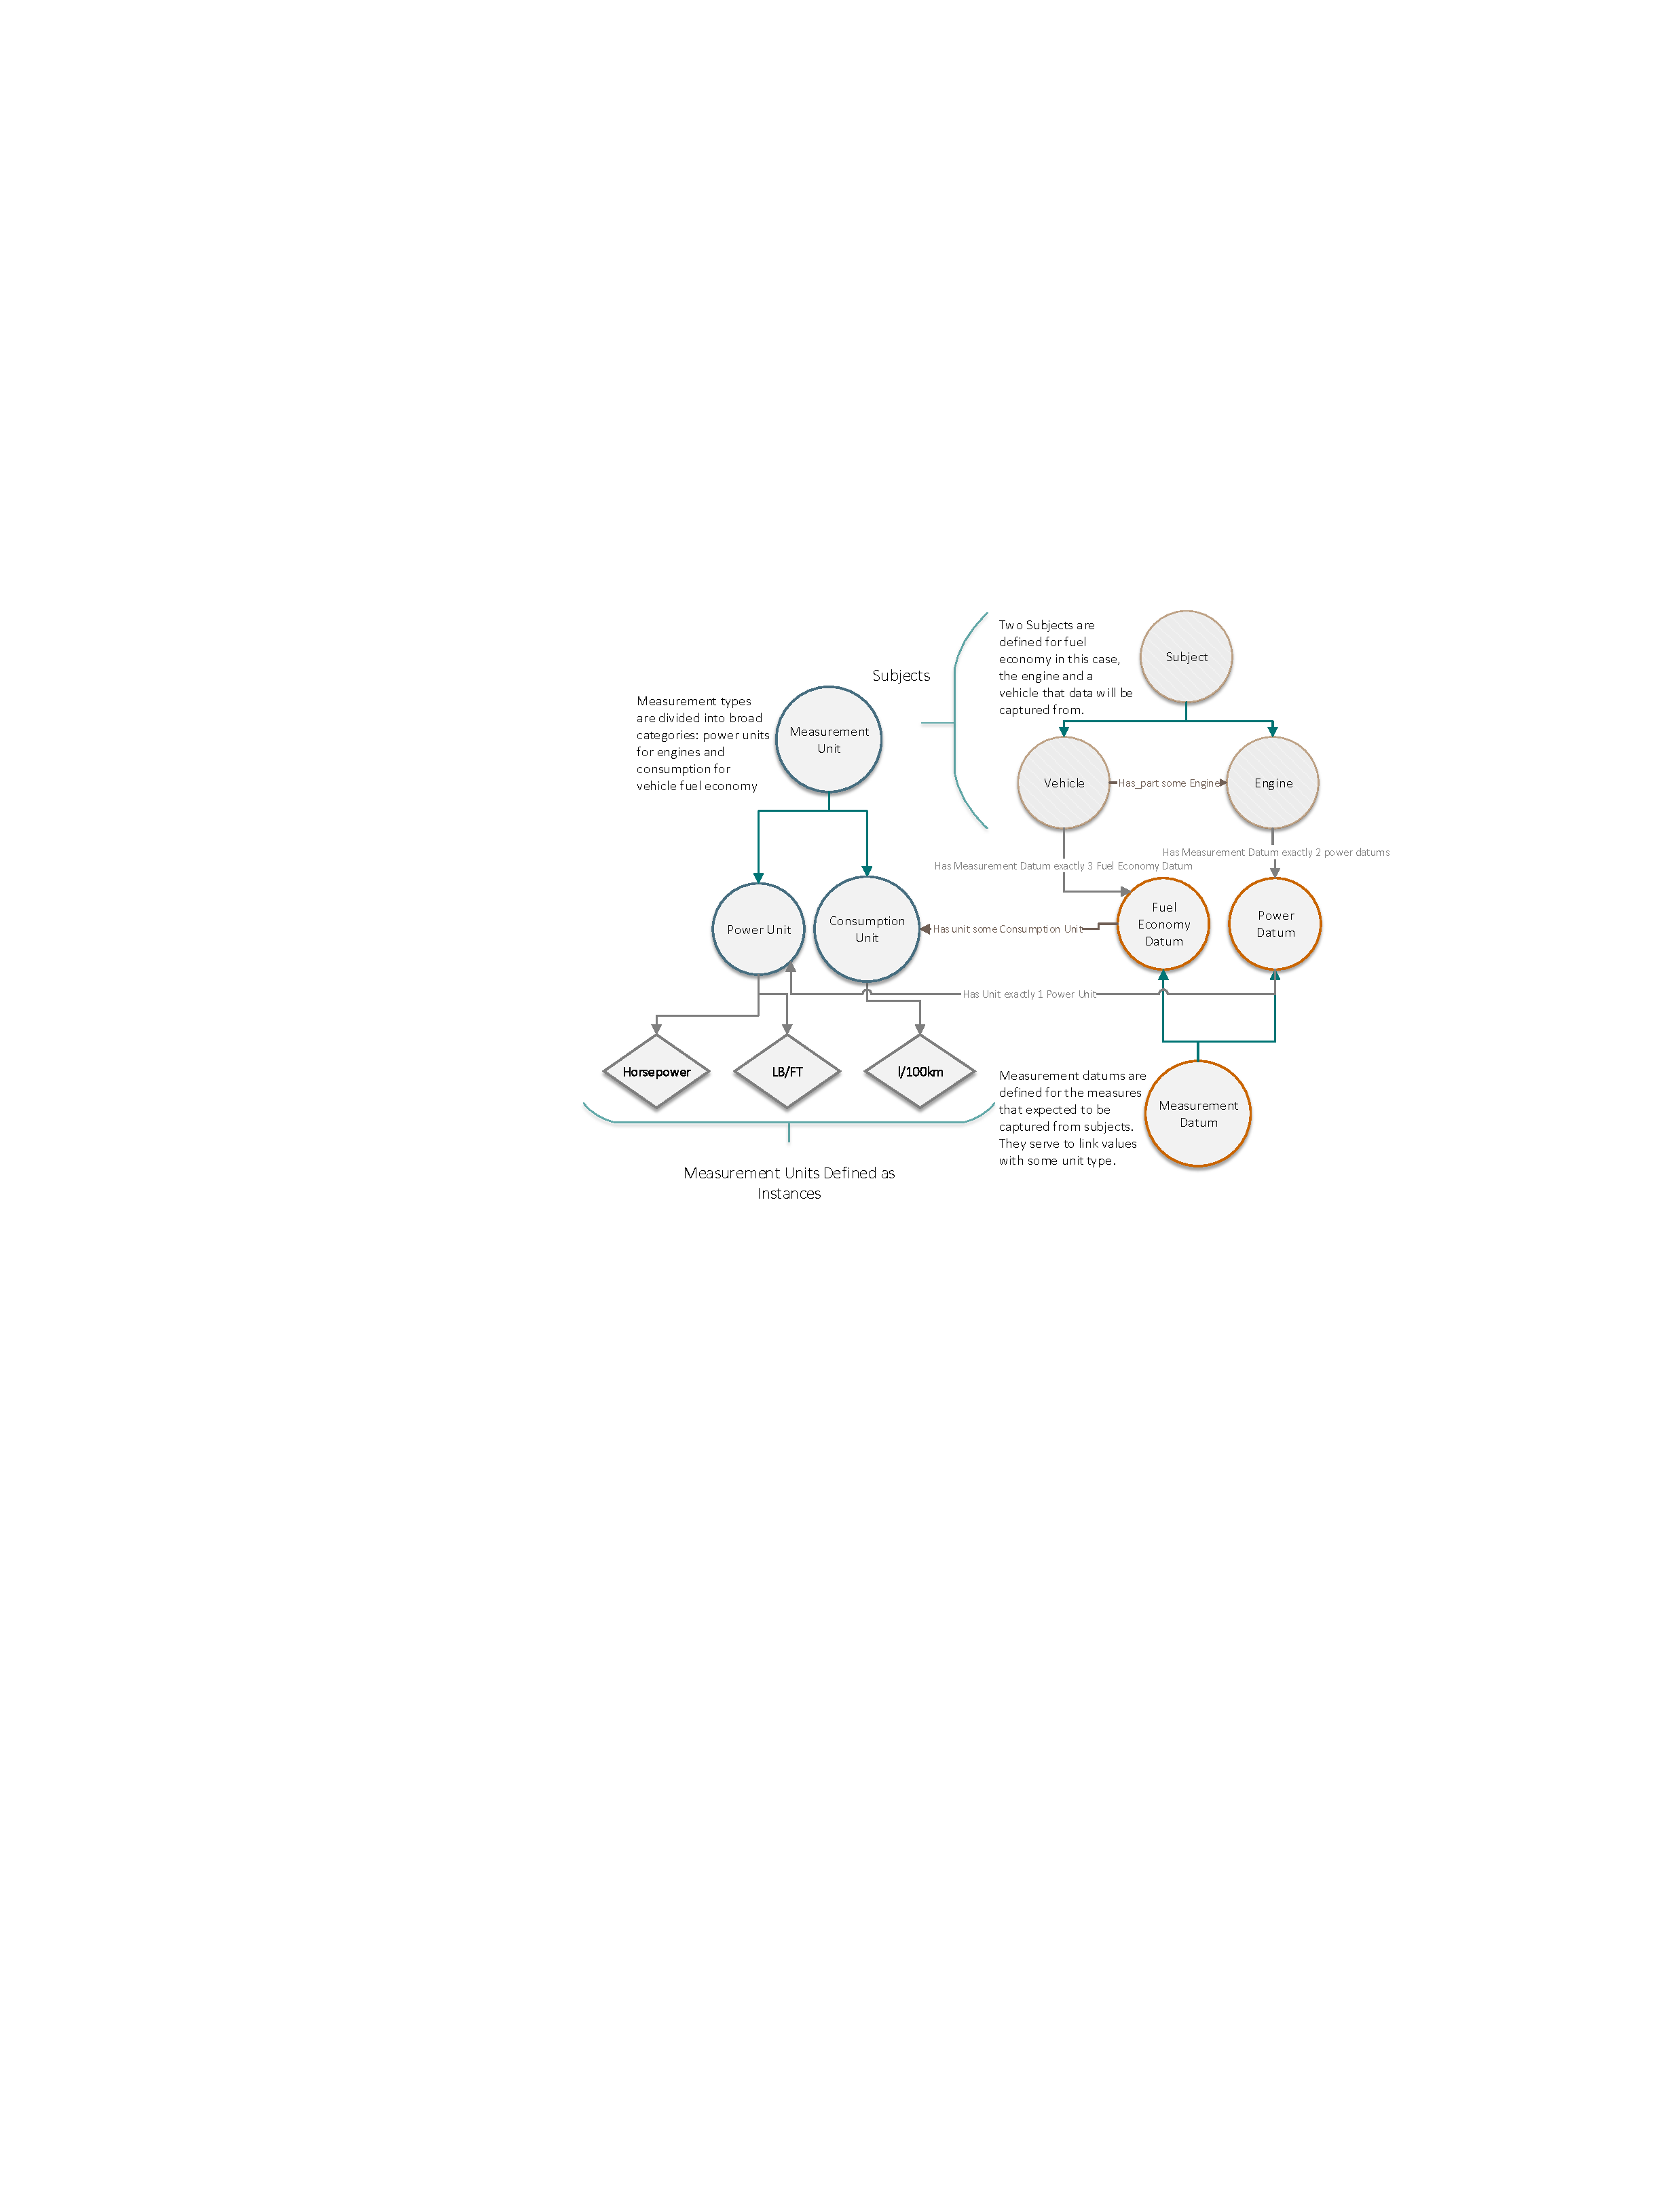
\includegraphics[height=4.45in]{Images/VehiclesExample}
\end{figure*}

\subsection{Tutorial AWS}
\label{sec:aws}

\noindent In the previous subsection (Section \ref{sec:tutorial1}), there were two LaTeX operations highlighted:
   \begin{enumerate}
   \item Including a figure (Figure \ref{fig:class})
   \item Including a bibliographic reference (in the caption of the diagram)
   \end{enumerate}

\section{\uppercase{Major Accomplishments and Contributions}}
\label{sec:accomplishments}

\noindent This section tells us what we should learn from your work.  Accomplishments are major elements of your project but contributions can be small items that you might not have planned for but had to do or learn to aid in your project work.

Feel free to add subsections to any of the sections specified in this document but do not remove any of the predefined sections.

\section{\uppercase{Future Work}}
\label{sec:future}

\noindent What could you have done better with this project?  If you were to continue this work (or if someone else decided to continue), what are the logical next steps for improvement or extension?

\section{\uppercase{Team Member Contributions}}
\label{sec:members}

\subsection{Team Member: Tyler Green}
\label{sec:tyler}

\noindent Have a subsection per team member.

\subsection{Team Member: Loui Zibdawi}
\label{sec:loui}

\noindent Have a subsection per team member.

\vfill
\bibliographystyle{apalike}
{\small \bibliography{ProjectReport}}


%\section*{\uppercase{Appendix}}
%
%\noindent If any, the appendix should appear directly after the
%references without numbering, and not on a new page. To do so please use the following command:
%\textit{$\backslash$section*\{APPENDIX\}}

\vfill
\end{document}

